\documentclass[12pt]{article}
\usepackage{graphicx}

\begin{document}
CSCI-4100 Assignment 2

Yichuan Wang 661414395\\
EXERCISES\\\\
1.8\\ %DONE
$v \leq 0.1$ means we get 1 red ball or 0 red ball. \\
P[1 red ball]: $10*(0.1)^9*0.9 = 9\times10^{-9}$\\
P[0 red ball]: $10^{-10}$\\
Answer: $9.1\times 10^{-9}$\\
1.9\\ %DONE
$u=0.9$, $v\leq0.1$, $|v-u|\geq0.8$
	$$P[|v-u|\geq0.8]\leq2e^{-2\times{0.8^2}\times10} = 5.52\times10^{-6}$$
The Hoeffding Bound result is greater than result from exercise 1.8\\\\
1.10\\
(a)\\%DONE
$u=0.5$ for these three coins.\\
(b)\\%DONE
$c_1$\\%DONE
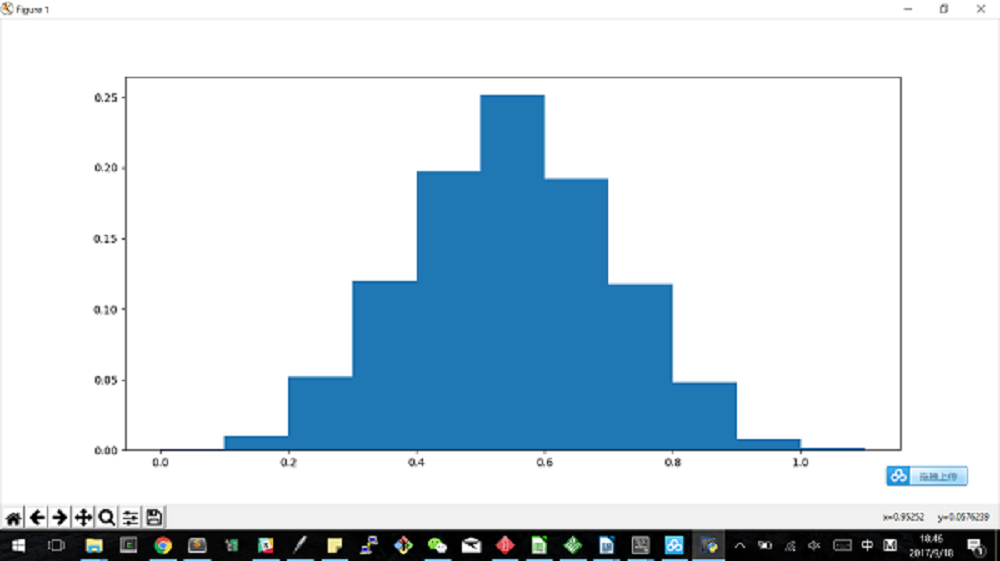
\includegraphics[scale=0.6]{c_1}\\\\
$c_{rand}$\\%DONE
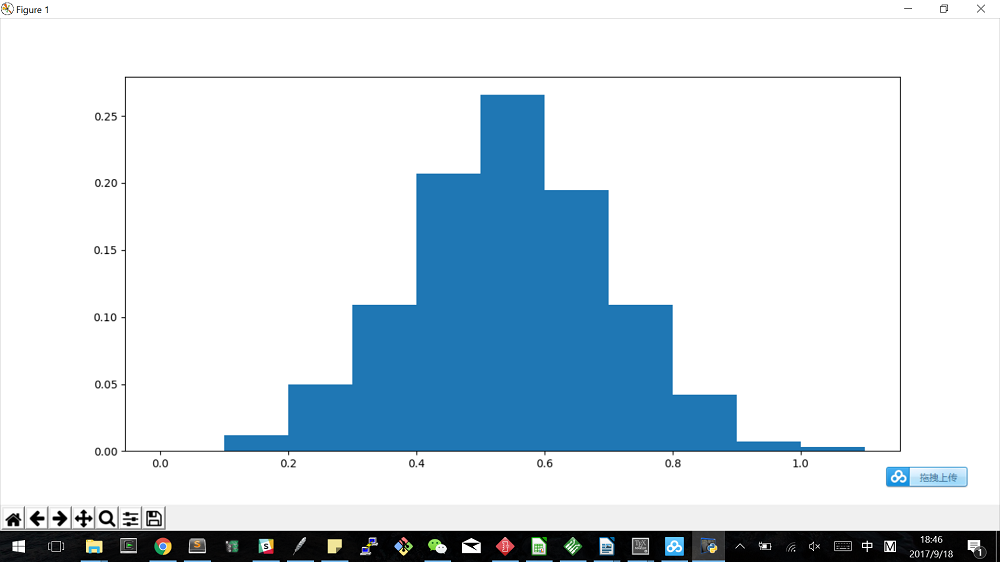
\includegraphics[scale=0.6]{c_rand}\\\\
$c_{min}$\\%DONE
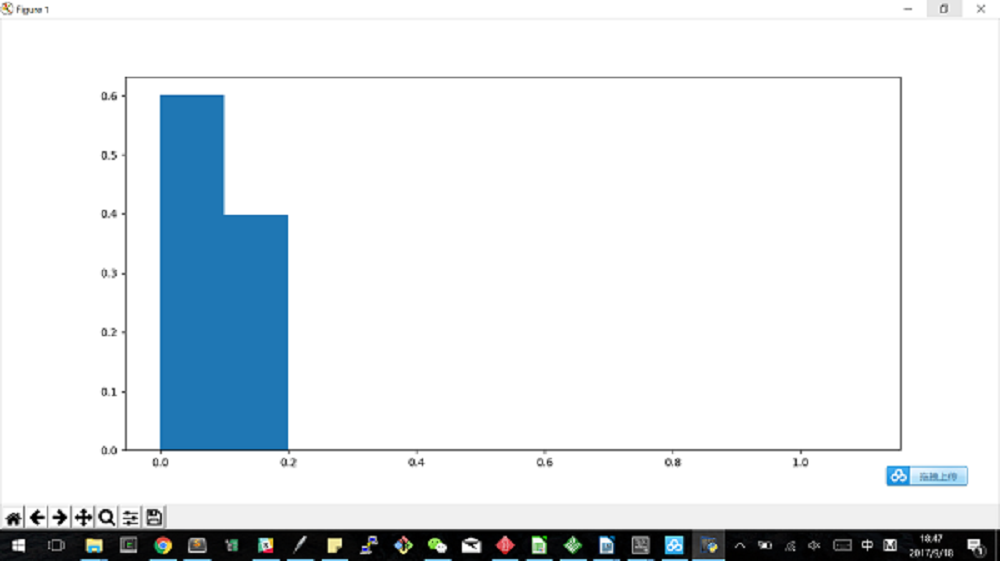
\includegraphics[scale=0.6]{c_min}\\\\
(c)\\
$c_1$\\
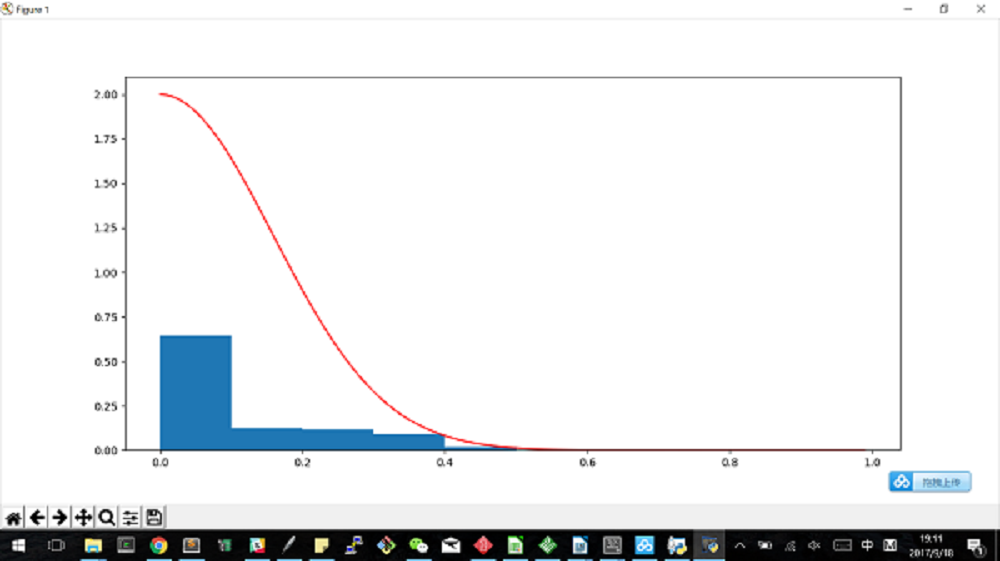
\includegraphics[scale=0.6]{c_1_c}\\\\
$c_{rand}$\\
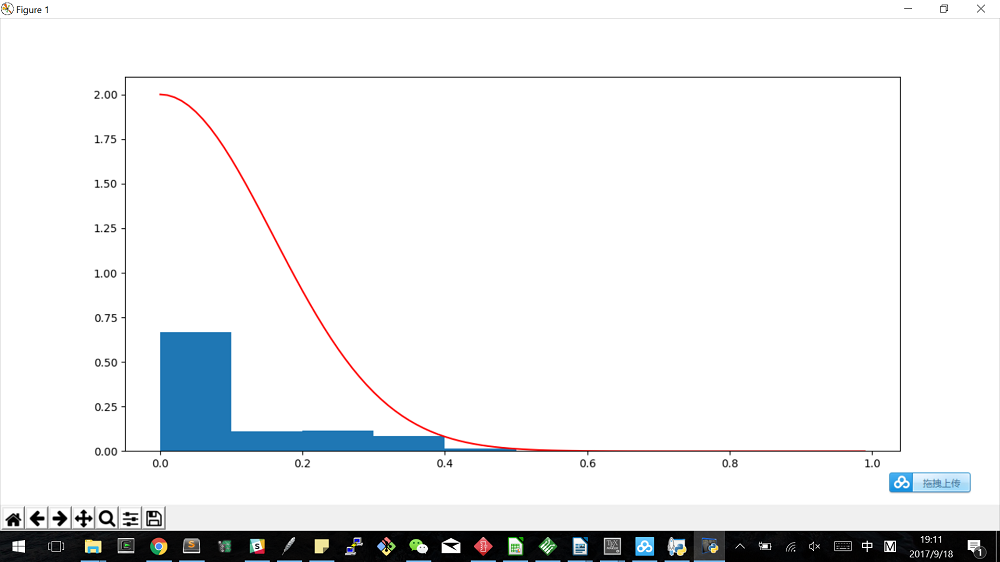
\includegraphics[scale=0.6]{c_rand_c}\\\\
$c_{min}$\\
\includegraphics[scale=0.6]{c_min_C}\\\\
(d)\\%DONE
The first coin and the random coin obey the Hoeffding Bound because they are fixed before sampling. The minimum coin doesn't obey the Hoeffding Bound because the selected coin is changed after sampling if a smaller $v$ is present from later sampling events.\\
(e)\\%DONE
There are 1000 bins, each having equal amount of green and red balls (u=0.5). We take ten balls from each bin and calculate $v$ based on our sampling result. Looking at the first flipped coin means we always look at the sampling result of bin no.1, which won't be affected by our sampling data. Same thing for the random selected bin; at each round we look at a fixed random bin for result. In this case, these two coin cases obey the Hoeffding Bound. The minimum coin case is such that we consider 1000 bins together and take the bin with minimum result. In this case our hypothesis is not fixed during data generation since we could always jump from one bin to another if the other bin has a lower $v$; so our result is not protected by Hoeffding Bound.\\

1.11\\
a) No.\\%DONE
b) Yes.\\%DONE
c)C is better than S when S choose h1, which will happen if there are 13 or more +1 from sampling. The probability is therefore$$\sum_{n=13}^{25}{25 \choose x} 0.9^k\times 0.1^{25-k} = 0.99999983791$$
d) There is no such p since the result from sample approximates the real result, and S chooses hypothesis based on sample. In this case S will always choose the better one between h1 and h2, and C will always choose the worse one. 

1.12\\%DONE
(c) is what I can promise. I cannot guarantee g’s performance, I cannot find a g that is likely to produce good performance, but I can check if the g I picked is likely to produce good performance.\\

PROBLEMS\\\\
1.3\\%DONE
(a) Since $w^*$ separates the data, all the data points are correctly classified. In this case all of $y_n(w^T*x_n)>0$, So $\rho>0$.\\\\  
(b)
$$w(t)=w(t-1)+y(t-1)x(t-1)$$
$$w^T(t)w^* = (w(t-1)+y(t-1)x(t-1)^Tw^*)=w^T(t-1)+y(t-1)w^{*T}x(t-1)$$
Since $\rho$ is the minimum of $y_nw^{*T}x_n$, we have $$y(t-1)w^{*T}x(t-1)\geq\rho$$. So we have $$w^T(t)w^*\geq w^T(t-1)w^* +\rho$$
Induction proof of $w^T(t)w^*\geq t\rho$:\\
Base Case: Iteration zero has $w(0)w^* = 0$ since $w(0)=0$, and $t\rho=0$ since $t=0$; we have: $$w(0)w^*=t\rho$$\\
Induction Step:\\
For iteration N ($t=N$), we have $$w(N)w^*\geq N\rho$$
We have proved $w^T(t)w^*\geq w^T(t-1)w^*+\rho$, by substituting in N we have $$w(N+1)^Tw^*\geq w(N)^Tw^*+\rho$$
Combine this equation with $w(N)w^*\geq N\rho$ we have $$w^T(N+1)w^*\geq (N+1)\rho$$\\
QED\\\\
(c)\\
$$w(t)=w(t-1)+y(t-1)x(t-1)$$
$$\parallel w(t)\parallel ^2 = \parallel w(t-1)\parallel ^2+\parallel x(t-1)\parallel ^2+2w^T(t-1)x(t-1)y(t-1)$$
$$w^T(t-1)x(t-1)y(t)<0 -- Missiclassfied$$
$$\parallel w(t)^2\parallel  \leq \parallel x(t-1)\parallel ^2+\parallel w(t-1)^2\parallel $$\\
QED\\\\
(d)\\
Base Case:\\
Iteration 0:
$$\parallel w(t=0)\parallel ^2=0=tR$$

Induction Step:\\
Assume iteration N is correct: $$\parallel w(N)\parallel ^2\leq NR^2$$
According to part (c), $$\parallel w(N+1)\parallel ^2 \leq \parallel w(N)\parallel ^2+\parallel x(N)\parallel ^2$$
Combine the result with assumption of iteration N we have $$\parallel w(N+1)\parallel ^2\leq NR^2+\parallel x(N+1)\parallel ^2$$
Since $R$ has the maximum absolute value among all $x_n$, we have $$\parallel x_n\parallel ^2\leq R^2$$
So we have $$\parallel w(N+1)\parallel ^2\leq NR^2+R^2$$
$$\parallel w(N+1)\parallel ^2\leq (N+1)R^2$$
QED\\\\
(e)\\
Take the square root of part(d)'s result: $$|w(t)|\leq \sqrt{t}R$$
Divide result of part(d) with the equation above:
$$\frac{w^T(t)}{{\parallel w(t)\parallel }w^*}\geq \frac{\sqrt{t}\rho}{R}$$
By moving $\rho$ and $R$ to the left side and take the square of both side of the equation, we get $$t\leq \frac{R^2\parallel w^*\parallel ^2}{\rho^2}$$
1.7\\%DONE
(a)\\%DONE
P[a coin has v=0](denoted by P[A]): $(1-u)^{10}$\\
P[at least 1 coin in n coins has v=0](denoted by $P[B_n]$): $1-(1-P[A])^n$\\\\
$u=0.05$:
$$P[A]=0.95^{10} = 0.5987 $$\\
$$P[B_1]=1-(1-P[A])^1 = 0.5987$$
$$P[B_{1000}]=1-(1-P[A])^{1000} = 1$$
$$P[B_{1000000}]=1-(1-P[A])^{1000000} = 1$$
$u=0.8$:\\
$$P[A]=0.2^{10} = 0.0000001024$$
$$P[B_1]=1-(1-P[A])^1 = 0.0000001024$$
$$P[B_{1000}]=1-(1-P[A])^{1000} = 0.0001024$$
$$P[B_{1000000}]=1-(1-P[A])^{1000000} = 0.0973$$
(b)\\%DONE
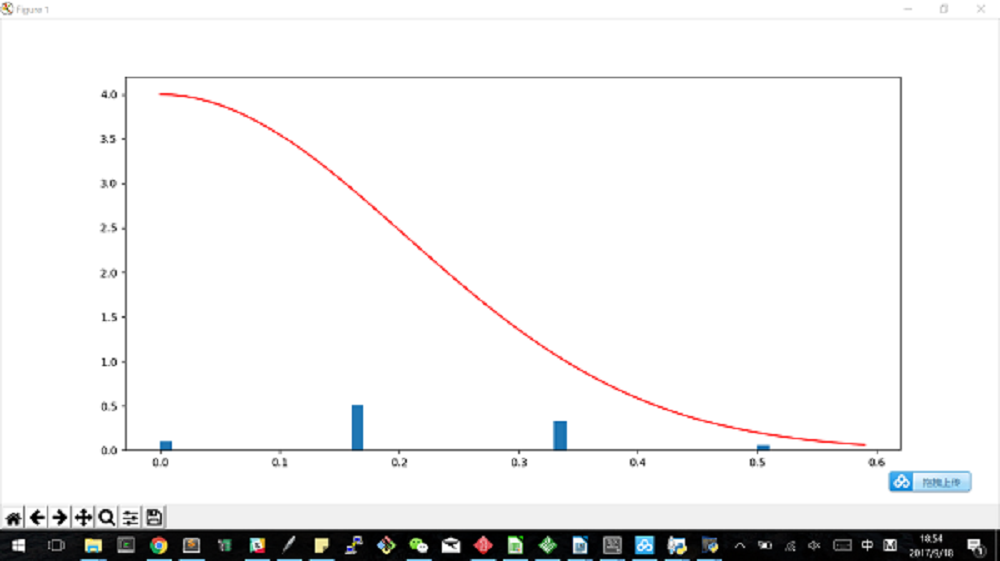
\includegraphics[scale=0.6]{1-7b}\\
The blue histogram is the probability of maximum error over two coins; the red curve is the Hoeffding Bound.\\ 
\end{document}